\documentclass[12pt, twoside]{article}
\usepackage[letterpaper, margin=1in, headsep=0.2in]{geometry}
\setlength{\headheight}{0.6in}
%\usepackage[english]{babel}
\usepackage[utf8]{inputenc}
\usepackage{microtype}
\usepackage{amsmath}
\usepackage{amssymb}
%\usepackage{amsfonts}
\usepackage{siunitx} %units in math. eg 20\milli\meter
\usepackage{yhmath} % for arcs, overparenth command
\usepackage{tikz} %graphics
\usetikzlibrary{quotes, angles}
\usepackage{graphicx} %consider setting \graphicspath{{images/}}
\usepackage{parskip} %no paragraph indent
\usepackage{enumitem}
\usepackage{multicol}
\usepackage{venndiagram}

\usepackage{fancyhdr}
\pagestyle{fancy}
\fancyhf{}
\renewcommand{\headrulewidth}{0pt} % disable the underline of the header
\raggedbottom
\hfuzz=2mm %suppresses overfull box warnings

\usepackage{hyperref}

\fancyhead[LE]{\thepage}
\fancyhead[RO]{\thepage \\ Name: \hspace{4cm} \,\\}
\fancyhead[LO]{BECA / Dr. Huson / Geometry\\*  Unit 2: Angles\\* 14 October 2022}

\begin{document}

\subsubsection*{2.7 Test: Angle measures}
\emph{Diagrams are not necessarily drawn to scale unless otherwise stated.}
\begin{enumerate}
\item Use the image of the protractor to measure each of the angles. \par \medskip
  \begin{tikzpicture}
    \draw[thick] (-3,0)--(0,0)--(3,0);
    \draw (4,0) arc (0:180:4);
    \draw[thick] (0,0) circle [radius=0.1];
    \foreach \x in {0,15,30,...,180}
      \node at (\x:3.4){\x};
    \foreach \x in {0,15,30,...,180}
      \draw (\x:3.7)--(\x:4);
    \foreach \x in {0,5,...,180}
      \draw (\x:3.9)--(\x:4);
    \draw[->,thick] (0,0)--(30:4.5)node[right]{m$\angle A = \rule{2cm}{0.1mm}$};
    \draw[->,thick] (0,0)--(50:4.5)node[right]{m$\angle B = \rule{2cm}{0.1mm}$};
    \draw[->,thick] (0,0)--(120:4.5)node[left]{m$\angle C = \rule{2cm}{0.1mm}$};
  \end{tikzpicture}

\item Find the measure of the angle in degrees with a protractor.
    \begin{flushright}
    \begin{tikzpicture}[scale=2]
      \draw[->, thick] (0,0)--(40:4);
      \draw[->, thick] (0,0)--(-10:5);
      \draw[fill] (40:3) circle [radius=0.025] node[above left ]{$D$};
      \draw[fill] (0,0) circle [radius=0.025] node[above left]{$E$};
      \draw[fill] (-10:4) circle [radius=0.025] node[above]{$F$};
    \end{tikzpicture}
    \end{flushright}

\item Given m$\angle ABD=30^\circ$, m$\angle DBC=40^\circ$. Calculate m$\angle ABC$.\vspace{0.5cm}
  \begin{flushright}
    \begin{tikzpicture}
      \draw[<->, thick] (40:5)--(0,0)--(6,0);
      \draw[->, thick] (0,0)--(70:4);
      \draw[fill] (70:3) circle [radius=0.05] node[left]{$A$};
      \draw[fill] (40:3) circle [radius=0.05] node[below right]{$D$};
      \draw[fill] (0,0) circle [radius=0.05] node[below]{$B$};
      \draw[fill] (4,0) circle [radius=0.05] node[below]{$C$};
      \node at (1.6,0.6){$40^\circ$};
      \node at (1.2,1.7){$30^\circ$};
    \end{tikzpicture}
    \end{flushright}

\newpage
\item Given the situation in the diagram, answer each question. Circle True or False. \vspace{0.25cm}
  \begin{multicols}{2}
    \begin{enumerate}
      \item T or F: $\angle RPT$ and $\angle SPU$ are \\adjacent angles. \bigskip
      \item T or F: $\angle TPS$ is an obtuse angle.\bigskip
      \item T or F: $\overrightarrow{PS}$ and $\overrightarrow{PT}$ are opposite rays.\bigskip
    \end{enumerate}
  \begin{tikzpicture}[scale=1]
    \draw[->, thick] (0,0)--(50:3.5);
    \draw[<->, thick] (-3,0)--(3,0);
    \draw[->, thick] (0,0)--(110:3);
    \draw[fill] (110:2.5) circle [radius=0.05] node[left ]{$S$};
    \draw[fill] (50:3) circle [radius=0.05] node[above left ]{$T$};
    \draw[fill] (0,0) circle [radius=0.05] node[below]{$P$};
    \draw[fill] (2,0) circle [radius=0.05] node[above]{$U$};
    \draw[fill] (-2,0) circle [radius=0.05] node[above]{$R$};
  \end{tikzpicture}
  \end{multicols}

\item As shown below, two lines intersect making four angles: $\angle 1$, $\angle 2$, $\angle 3$, and $\angle 4$.
  \begin{center}
  \begin{tikzpicture}[scale=0.6, rotate=15]
    \draw[<->, thick] (0,-1.5)--(10,1.5);
    \draw[<->, thick] (2,3.5)--(7,-3.5);
    \node at (3,.4){1};
    \node at (6,-.6){3};
    \node at (5,1){2};
    \node at (4,-1){4};
  \end{tikzpicture}
  \end{center}
  \begin{enumerate}
    \item Given that m$\angle 1= 65^\circ$, find m$\angle 3=$ \rule{2.5cm}{0.15mm} \bigskip
    \item $\angle 2 \cong$ \rule{2.5cm}{0.15mm} \bigskip
    \item True or false, $\angle 1$ and $\angle 4$ are complementary angles. \rule{3cm}{0.15mm}
\end{enumerate} \vspace{0.5cm}

\item 
  \begin{enumerate}
    \item Given, the diagram below. Name a right angle:  \rule{4cm}{0.15mm}  \bigskip
    \item Name an angle that is complementary to $\angle AOB$: \rule{4cm}{0.15mm} \bigskip
    \item Name the angle that is opposite to $\angle DOE$: \rule{4cm}{0.15mm}
  \end{enumerate}
  \begin{center}
  \begin{tikzpicture}[scale=1.1, rotate=20]
    \draw[<->, thick] (-25:5)--(0,0)--(155:5);
    \draw[<->, thick] (-5,0)--(5,0);
    \draw[->, thick] (0,0)--(0,3);
    \draw (0,0)++(0.3,0)--++(0,0.3)--+(-0.3,0);
    \draw[fill] (155:3) circle [radius=0.05] node[below left]{$B$};
    \draw[fill] (-4,0) circle [radius=0.05] node[below]{$A$}; 
    \draw[fill] (0,0) circle [radius=0.05] node[below left]{$O$};
    \draw[fill] (0,2) circle [radius=0.05] node[left]{$C$};
    \draw[fill] (4,0) circle [radius=0.05] node[below]{$D$};
    \draw[fill] (-25:2) circle [radius=0.05] node[below]{$E$};
  \end{tikzpicture}
  \end{center}

\newpage
\emph{For full credit on these three problems, start with an equation and check your solution.}
\item Given m$\angle BAC = 4x+2$ and m$\angle CAD = 3x+3$, m$\angle BAD=75^\circ$. Find m$\angle BAC$.
  \begin{flushright}
  \begin{tikzpicture}[scale=1]
    \draw[<->, thick] (-10:4)node[above left]{$B$} 
    --(0,0)node[left]{$A$}
    --(-52:5)node[above right]{$C$};
    \draw[->, thick] (0,0)--(-85:4)node[above left]{$D$};
    \node at (2,-1){$4x+2$};
    \node at (1,-2.5){$3x+3$};
  \end{tikzpicture}
  \end{flushright} \vspace{1.5cm}

\item As shown below, two lines intersect making four angles: $\angle 1$, $\angle 2$, $\angle 3$, and $\angle 4$. Given that m$\angle 1= x+32$ and m$\angle 3=2x-8$, find m$\angle 1$.
  \begin{flushright}
    \begin{tikzpicture}[scale=1, rotate=0]
      \draw[<->, thick] (1,-1)--(8,1);
      \draw[<->, thick] (3,2)--(6,-2);
      \node at (2,.3){m$\angle 1= x+32$};
      \node at (6.5,-.3){m$\angle 3=2x-8$};
      \node at (5,1){2};
      \node at (4,-1){4};
    \end{tikzpicture}
    \end{flushright} \vspace{1cm}

\item An angle bisector is shown below, with $\overrightarrow{PR}$ bisecting $\angle QPS$. Given m$\angle QPR = 5x-8$ and m$\angle RPS = 3x+20$, find m$\angle QPS$.
    \begin{flushright}
    \begin{tikzpicture}[scale=0.6, rotate=30]
      \draw[<->, thick] (230:5)node[left]{$Q$} 
      --(0,0)node[above right]{$P$}
      --(110:6)node[above right]{$S$}--(110:7);
      \draw[->, thick] (0,0)--(170:7)node[below right]{$R$};
    \end{tikzpicture}
    \end{flushright}

\newpage
\subsubsection*{Do Not Solve! \\
Model the situation with an equation. Circle where it states what to find.}

\item In the diagram below $\angle AOB = 2x$ and $\angle COB = 5x+20$. Find m$\angle AOB$. \vspace{0.25cm}
\begin{flushright}
\begin{tikzpicture}[scale=0.7, rotate=20]
\draw[<->, thick] (-25:5)--(0,0)--(155:5);
\draw[<->, thick] (-5,0)--(5,0);
\draw[->, thick] (0,0)--(0,4);
\draw (0,0)++(0.3,0)--++(0,0.3)--+(-0.3,0);
%\draw[fill] (-1,2.5) circle [radius=0.05] node[left ]{$B$};
\draw[fill] (155:3) circle [radius=0.05] node[below left]{$B$};
\draw[fill] (-4,0) circle [radius=0.05] node[below]{$A$}; 
\draw[fill] (0,0) circle [radius=0.05] node[below]{$O$};
\draw[fill] (0,3) circle [radius=0.05] node[left]{$C$};
\draw[fill] (4,0) circle [radius=0.05] node[below]{$D$};
\draw[fill] (-25:2) circle [radius=0.05] node[below]{$E$};
\end{tikzpicture}
\end{flushright}

\item Two lines intersect making four angles: $\angle 1$, $\angle 2$, $\angle 3$, and $\angle 4$. Given that m$\angle 1= 6x+28$ and m$\angle 3=8x+12$. Find m$\angle 1$.
\begin{flushright}
\begin{tikzpicture}[scale=0.5, rotate=-10]
\draw[<->, thick] (0,-1.5)--(10,1.5);
\draw[<->, thick] (2,2)--(7,-2);
\node at (3,.4){1};
\node at (6,-.6){3};
\node at (5,1){2};
\node at (4,-1){4};
\end{tikzpicture}
\end{flushright}

\item In the diagram below $\angle AOB = 10x+3$ and $\angle DOE = 63^\circ$. Find $x$. \vspace{0.25cm}
\begin{flushright}
\begin{tikzpicture}[scale=0.7, rotate=-20]
\draw[<->, thick] (-55:3)--(0,0)--(125:4);
\draw[<->, thick] (-5,0)--(5,0);
\draw[->, thick] (0,0)--(0,4);
\draw (0,0)++(0.3,0)--++(0,0.3)--+(-0.3,0);
\draw[fill] (125:3) circle [radius=0.05] node[below left]{$B$};
\draw[fill] (-4,0) circle [radius=0.05] node[below]{$A$}; 
\draw[fill] (0,0) circle [radius=0.05] node[below left]{$O$};
\draw[fill] (0,3) circle [radius=0.05] node[left]{$C$};
\draw[fill] (4,0) circle [radius=0.05] node[below]{$D$};
\draw[fill] (-55:2) circle [radius=0.05] node[left]{$E$};
\end{tikzpicture}
\end{flushright}

\item Given that m$\angle 2= 10x-20$ and m$\angle 3=3x+5$ as shown in the diagram, find m$\angle 2$.
\begin{flushright}
\begin{tikzpicture}[scale=0.5, rotate=-30]
\draw[<->, thick] (0,-1.5)--(10,1.5);
\draw[<->, thick] (2,2)--(7,-2);
\node at (3,.4){1};
\node at (6.3,-.5){3};
\node at (5,1){2};
\node at (4,-1){4};
\end{tikzpicture}
\end{flushright}

\end{enumerate}
\end{document}